\section{I/O Subsystem}

\noindent
The \textbf{Simple Operating System(SOS)}, also provides an abstraction of the file systems and the corresponding read, write, open, close operations on it to the userspace using the UNIX semantics
wherein the corresponding calls on an arbitrarily provided path goes back to the sos system call management loop, which in turn creates a generalized file interface for the particular being opened and store a pointer to it in the 
the file allocation table for its processes struct and then the specific file interface function call makes a call to the server loop with setting the correct call\_context makes a call to the file server loop waiting on the specific endpoint for the user input to appear 
which in turn spawns of the request to the correct asynchronous nfs call using the libnfs interface which makes a call to the correct callback corresponding to each of the calls that the user makes in.
\\

\noindent The SOS in general supports the serial and the console operation semantics using the libserial interface and the generalized files are initialized and managed using the 
Network file system(\textbf{NFS}) which are both dealt with asynchronously and corresponding to each request we destroy the reply object after replying back correctly
inside the corresponding callback for the libnfs asynchronous call.
\\

\noindent
Currently we make an assumption that there can only be 1024 files open for a particular process at any time, which is represented by FD\_MAX inside 
process.h for the process file descriptor table represented by file\_interface fd\_table[FD\_MAX] inside the process\_data struct.
\\

\subsection{Generalized File Interface}


\begin{figure}[h]
    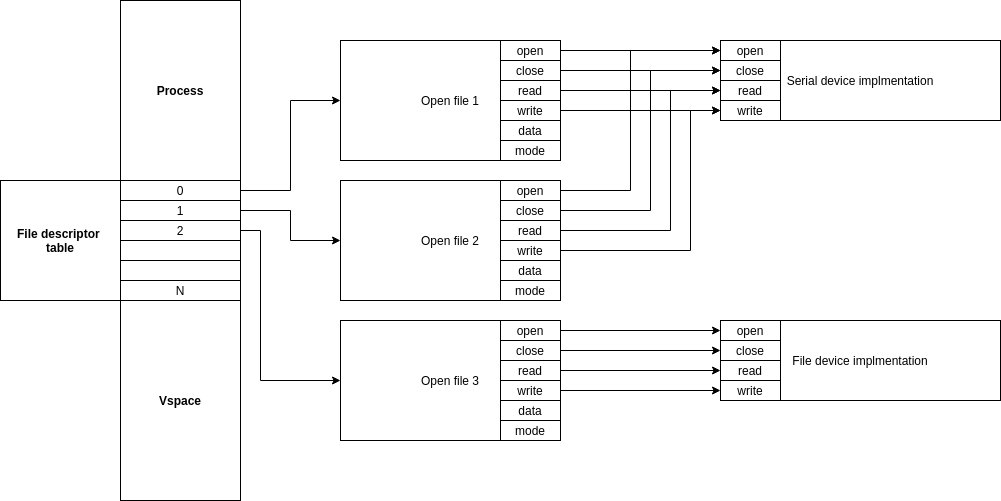
\includegraphics[width=\linewidth]{file_interface.png}
    \caption{File interface overview}
    \label{fig:file_interface}
\end{figure}

We use this generalized file interface inside \textbf{SOS} for any of the files that are created,

\noindent
\{ \par
    \textbf{int (*open)(struct fi\_inner * interface, const char * filename, sos\_thread\_t * thread);} \par
    \textbf{int (*read)(struct fi\_inner * interface, char * buffer, int len, bool * stop);} \par
    \textbf{int (*write)(struct fi\_inner * interface, const char * buffer, int len, bool * stop);} \par
    \textbf{int (*close)(struct fi\_inner * interface);} \par
    \textbf{int mode;} \par
    \textbf{void * data;} \par
    \noindent
\} \\

\noindent
We store a reference to each of the file interfaces whenever a file is opened inside the processes vspace(as shown in the figure above) using a file descriptor table,where in
the index value inside the processes vspace represents the file descriptor allocated to the that particular file.
\\

\noindent
For the purpose of initializing an entry of any particular type of device we compare the path name given to the SOS for creating a file and if it is "console' then we call our specialized serial interface initialization function called as 
make\_serial\_device(interface) which initializes a new serial interface over which we can call its interface specific open, read, write and close and other file operation semantics and if 
the path for the file being created is anything other than "console" then we make a call to the make\_file\_device(interface) to initialize the file interface.
To handle the read and write permissions for the file when we are creating a file interface itself we store the 'mode' with which the file was created in
the file interface struct corresponding to that file itself and whenever we are reading and writing we make sure that the the readable files are not been written and not changed up.
\\

\subsection{File descriptor allocation}

\noindent
For the purposes of the file descriptor allocation we use a bitmap structure inside util.c representing the which of the indexes inside the fd\_table for the process are currently storing the reference to an open file.
We find the first free bit inside our bitmap represented by bitfield\_fd[BITFIELD\_MAX], where BITFIELD\_MAX is (1024/8) as we need each entry inside it will represent 8 bits for the 1024 files that can potentially be open at any time.
We make an assumption that the first 3 file descriptors will always be allocated for STDIN, STOUT AND STDERR and any other file being opened will only be given a file descriptor from 3 onwards.
The bitmap structure helps us to find the first free bit/ first free id that can be allocated any process quite quickly in comparison to looping through the entire array of the 
File interfaces and therefore considering this aspect itself we have tried to incorporate a bitmap for each process to help us with the file descriptor allocation.
Whenever we close the file the bit value corresponding to its file descriptor is reset to 0.
\\

\subsection{Serial Interface}

\begin{figure}[h]
    \centering
    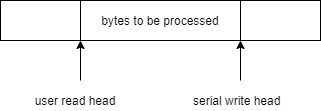
\includegraphics[width=75mm]{serial_buffer.png}
    \caption{Console circular buffer}
    \label{fig:serial_buffer}
\end{figure}

\noindent
The serial console is a many-writer, single-reader device. Therefore
when a process opens the console device for reading, it will block if there
is already another device reading the console. Processes opening the console
just for writing will be able to open it without blocking. While no one has
the console opened the console for reading, any bytes coming in through the 
console handler are dropped.
\\

\noindent
When the console is opened for reading, the serial handler will place received
bytes into the circular buffer. When a user tries to read a number of bytes
from the console, they are read out of this buffer. In this way, a user will
be able to read all the bytes typed in the console after they opened it for
reading. If there are no newlines in the buffer, or if the the number of bytes
in the buffer is smaller than requested by the user, the SOS thread processing
the user's request will block until more input is received from the console.
The circular buffer makes no attempt to prevent the write head moving past
the read head. If the user is unable to process input to the console fast
enough, some bytes will be dropped.
\\


\subsection{File server}

For the purpose of handling the file management system calls we separately create file server thread initially when the system is 
initialized which is waiting on a separate endpoint inside a server loop waiting for a request from the user. When we initialize the system we also a create a separate notification object 
called load\_ntfn which is used to notify the process management thread which waits on the load\_ntfn until the libnfs is mounted and is signalled back when inside network.c  the nfs\_mount\_async signals on the same notification object as soon as it is mounted in. The file server thread is always waiting on a separate endpoint for any user requests which are given to it from the syscall management specific 
SOS thread or by directly calling into the file interface specific functions which directly makes a call into the server loop. The specific system call primarily makes a call to the specific file handling function defined in file.h which sets up the call context for the server loop and when the server loop acquires a request on its endpoint then
then based on the type set in the call\_context it makes in a call to the specific nfs library asynchronous call with the correct parameters and after it correctly deals with the correctly dealing with file management with regards to the call made inside the libnfs directory then it makes in a call to the callback functions corresponding to the asynchronous calls which checks in the errors received if any by the libnfs function 
and then reply back the reply using the reply object passed in as the call context and then the reply object is freed as the sever loop creates a new reply object corresponding to each call by saving the previous reply object each time inside the call context structure unless it is handling a notification.
The callback specific information which is created is sent back to the fie interface specific functions which receives back the data from the callback and then set the data of the file interface passed in with the data returned from the specific callback and this how we 
persist the information for the file\ interface which is passed in, and to persist the information for the libnfs file which is opened in we use the structure open\_file\_t which stores a pointer to the nfsfh which is stored in the structure whenever a new nfs file is created and its cache position is updated with writes to get a better write performance for the overall system.








